\documentclass[../../main.tex]{subfiles}

\begin{document}
    \section{Implementing Symbol Manipulation in MLPs}
    When specifying the structure of a neural network, we restrict our hypothesis class, i.e. we restrict the possible mappings from the input to the output space. Furthermore, we also encode a \emph{bias} into the network, i.e. a certain tendency to prefer some mappings over others.

    TODO: example interpolation etc.

    Our goal is to encode the premised human bias for UQOTOMs (at least for certain tasks) to MLPs in order to achieve good generalization of these models. We hope that by examining successful models we might be able to draw conclusions to the inner mechanisms of the human brain.
    
    Understanding the bias and learning behavior of multilayer perceptrons is rather difficult, which is why empirical testing is used to assess different architectures.
    
    \subsection{MLPs with Linear Activation Functions}
    When restricting our models to only using linear activation function, though, we can infer some information:
    
    \begin{proposition}
        \label{proposition:linear_mlp}
        The hypothesis class of a MLP with linear activation functions is restricted to linear functions $f: \mathbb{R}^m \mapsto \mathbb{R}^n$, i.e. there exists a matrix $\bm{M} \in \mathbb{R}^{n \times m}$ s.t. $f(\bm{v}) = \bm{Mv}$.
    \end{proposition}
    \begin{proof}
        Consider a multi-layer perceptron with $L$ layers and linear activation functions $\phi(x) = \alpha x$. Let the input be $\bm{v} \in \mathbb{R}^m$, and let each layer $i$ have a weight matrix $\bm{W}^{(i)}$. The output of the network is:
        \[
        f(\bm{v}) = \phi\left( \bm{W}^{(L)} \phi\left( \bm{W}^{(L-1)} \phi\left( \cdots \phi\left( \bm{W}^{(1)} \bm{v} \right) \cdots \right) \right) \right) \quad ,
        \]
        where $\phi$ is applied element-wise. Since $\phi(x) = \alpha x$, this simplifies to:
        \[
        f(\bm{v}) = \alpha^L \bm{W}^{(L)} \bm{W}^{(L-1)} \cdots \bm{W}^{(1)} \bm{v} \quad .
        \]
        Let $\bm{M} = \alpha^L \bm{W}^{(L)} \bm{W}^{(L-1)} \cdots \bm{W}^{(1)} \in \mathbb{R}^{n \times m}$. Then $f(\bm{v}) = \bm{M} \bm{v}$, which is a linear function. Thus, the hypothesis class is restricted to linear mappings from $\mathbb{R}^m$ to $\mathbb{R}^n$.
    \end{proof}

    \begin{remark}
        This proposition also holds when allowing $\alpha$ to vary by layer, or even with every node.
    \end{remark}

    \begin{lemma}
        \label{lemma:injective_matrix}
        Let $\bm{M} \in \mathbb{R}^{n \times m}$ be a matrix inducing the mapping $f(\bm{v}) \coloneqq \bm{Mv}$. Then we have
        \[
            f \text{ injective} \iff \operatorname{rank} \bm{M} = m \quad .
        \]
    \end{lemma}
    \begin{proof}
        The function $f$ is injective iff $\ker(\bm{M}) = \{\bm{0}\}$:
        
        '$\implies$' is trivial. For '$\impliedby$', consider the contraposition '$f$ is not injective $\implies \ker(\bm{M}) \neq \{\bm{0}\}$'. Since $f$ is not injective, there must be $\bm{u}, \bm{v} \in \mathbb{R}^m$ with $\bm{u} \neq \bm{v}$ s.t. $\bm{Mu} = \bm{Mv}$. Hence, $\bm{M}(\bm{u}-\bm{v}) = \bm{0}$, and thus $(\bm{u}-\bm{v}) \in \ker{\bm{M}}$. Note that $(\bm{u}-\bm{v}) \neq \bm{0}$.

        Now, by the rank-nullity theorem, we have:
        \[
        \dim(\ker(\bm{M})) + \operatorname{rank}(\bm{M}) = m \quad .
        \]
        Finally, we see that
        \[
            \operatorname{rank}(\bm{M}) = m \iff \dim(\ker(\bm{M})) = 0 \iff \ker(\bm{M}) = \{\bm{0}\} \iff f \text{ injective} \quad .
        \]
    \end{proof}

    \begin{corollary}
        A MLP with only one input node and linear activations is forced to learn either $f: \mathbb{R} \mapsto \mathbb{R}^n, f(x) \equiv \bm{0}$ or an UQOTOM.
    \end{corollary}
    \begin{proof}
        Based on proposition~\ref{proposition:linear_mlp} we know that $f$ can be written as $f(x) = \bm{v} x$ for some $v \in \mathbb{R}^{n \times 1}$. Furthermore, based on lemma~\ref{lemma:injective_matrix} we know that $f \text{ injective} \iff \operatorname{rank}\bm{v} = 1$. Since $\bm{v}$ is a vector, we have $\operatorname{rank}\bm{v} = 1 \iff \bm{v} \neq \bm{0}$.

        Hence, for $\bm{v} \neq \bm{0}$ we have that $f$ is injective. When restricting the image domain accordingly we also have that $f$ is surjective, and hence UQOTOM.

        On the other hand, if $\bm{v} = \bm{0}$, then $f(x) \equiv \bm{0}$.
    \end{proof}

    \begin{remark}
        If a MLP with linear activations has multiple input nodes, it will depend on the properties of matrix $\bm{M}$ whether or not the MLP implements an UQOTOM based on lemma~\ref{lemma:injective_matrix}.

        For example, consider the mapping
        \[
            f: \mathbb{R}^2 \mapsto \mathbb{R}^2, \bm{v} \mapsto
            \begin{pmatrix*}
                1 & 1 \\
                0 & 0 \\
            \end{pmatrix*}
            \bm{v} \quad .
        \]
        It is not injective, since $f
        \begin{pmatrix*}
            1 \\
            0 \\
        \end{pmatrix*} = f
        \begin{pmatrix*}
            0 \\
            1 \\
        \end{pmatrix*}
        =
        \begin{pmatrix*}
            1 \\
            0 \\
        \end{pmatrix*}$. Such a mapping can be implemented by the MLP depicted in figure~\ref{fig:non_injective_linear_mlp}.

        \begin{figure}[h]
            \centering
            \begin{tikzpicture}[
                neuron/.style={circle, draw=black, minimum size=1cm},
                layer/.style={node distance=1.5cm and 2cm},
                every edge/.style={draw,->,thick}
            ]

            % Input Layer
            \node[neuron] (I1) at (0,1.5) {$v_1$};
            \node[neuron] (I2) at (0,-1.5) {$v_2$};

            % Output Layer
            \node[neuron, right=4cm of I1] (O1) {$f_1$};
            \node[neuron, right=4cm of I2] (O2) {$f_2$};

            % Connections with weights
            \draw (I1) edge node[pos=0.3, above] {$1$} (O1);
            \draw (I1) edge node[pos=0.3, above] {$0$} (O2);
            \draw (I2) edge node[pos=0.3, below] {$1$} (O1);
            \draw (I2) edge node[pos=0.3, below] {$0$} (O2);
            \end{tikzpicture}
            \label{fig:non_injective_linear_mlp}
            \caption{Simple MLP with linear activations implementing a non-injective mapping.}
        \end{figure}
    \end{remark}

    \subsection{MLPs with Non-Linear Activation Functions}
    In order to learn not just linear mappings, MLP typically employ non-linear sigmoidal activation functions, like the logistic function $\sigma(x) \coloneqq \frac{1}{1+e^{-x}}$ or $\tanh(x) \coloneqq \frac{e^x - e^{-x}}{e^x + e^{-x}}$.

    \begin{figure}[h]
    \centering
        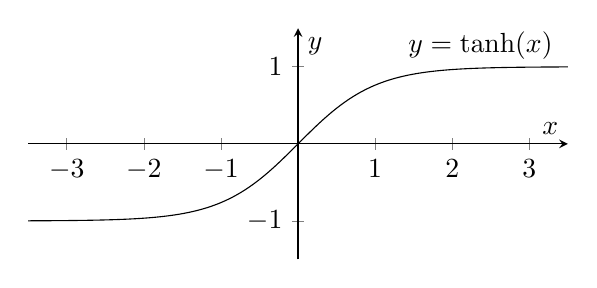
\begin{tikzpicture}[>=stealth]
            \begin{axis}[
                axis equal image,
                xmin=-3.5,xmax=3.5,
                ymin=-1.5,ymax=1.5,
                axis x line=middle,
                axis y line=middle,
                axis line style=->,
                xlabel={$x$},
                ylabel={$y$},
                ]
                \addplot[no marks,black,-] expression[domain=-5:5,samples=1000]{tanh(x)} 
                            node[pos=0.65,anchor=south west, yshift=0.1cm]{$y=\tanh(x)$}; 
            \end{axis}
        \end{tikzpicture}
        \caption{Plot of the function $y=\tanh(x)$.}
    \end{figure}

    As it turns out, the analysis of such MLPs with non-linear activations is much harder.

    \begin{example}
        MLPs with non-linear activations like $\tanh(x)$ can represent non-injective functions (other than $f(x) \equiv \bm{0}$) even when only using one input node.
        
        For instance, the MLP depicted in figure~\ref{fig:non_injective_mlp_single_input} implements the non-injective mapping depicted in figure~\ref{fig:non_injective_function}.

        \begin{figure}[h]
            \centering
            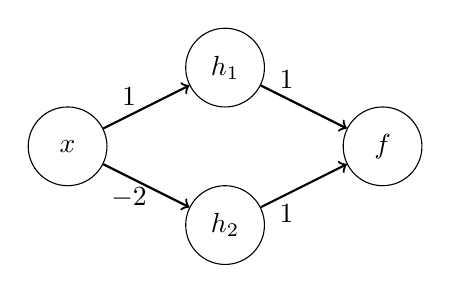
\begin{tikzpicture}[
                    neuron/.style={circle, draw=black, minimum size=1cm},
                    layer/.style={node distance=1.5cm and 2cm},
                    every edge/.style={draw,->,thick}
                ]

                % Input Layer
                \node[neuron] (I1) at (0,0) {$x$};

                \node[neuron] (H1) at (2, 1) {$h_1$};
                \node[neuron] (H2) at (2, -1) {$h_2$};

                % Output Layer
                \node[neuron] (O1) at (4, 0) {$f$};

                % Connections with weights
                \draw (I1) edge node[pos=0.3, above] {$1$} (H1);
                \draw (I1) edge node[pos=0.3, below] {$-2$} (H2);
                \draw (H1) edge node[pos=0.3, above] {$1$} (O1);
                \draw (H2) edge node[pos=0.3, below] {$1$} (O1);
            \end{tikzpicture}
            \caption{Simple MLP using $\tanh(x)$ activation implementing a non-injective mapping.}
            \label{fig:non_injective_mlp_single_input}
        \end{figure}

        \begin{figure}[h]
        \centering
            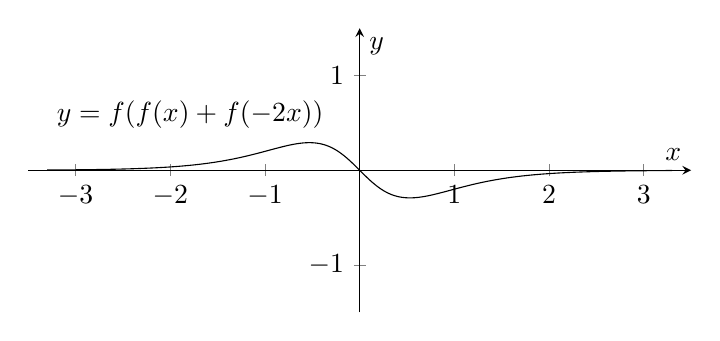
\begin{tikzpicture}[>=stealth]
                \begin{axis}[
                    axis equal image,
                    width=10cm,
                    xmin=-3.5,xmax=3.5,
                    ymin=-1.5,ymax=1.5,
                    axis x line=middle,
                    axis y line=middle,
                    axis line style=->,
                    xlabel={$x$},
                    ylabel={$y$},
                    ]
                    \addplot[no marks,black,-] expression[domain=-3.3:3.3,samples=1000]{tanh(tanh(x) + tanh(-2 * x))} 
                                node[pos=0,anchor=south west, yshift=0.4cm]{$y=f(f(x) + f(-2x))$}; 
                \end{axis}
            \end{tikzpicture}
            \caption{Plot of the function $y=f(f(x) + f(-2x))$ with $f(x) \coloneqq \tanh(x)$.}
            \label{fig:non_injective_function}
        \end{figure}
    \end{example}
\end{document}
